% Implementation chart of the eICU reproducibility arm of the attributability
% analysis (attribution plan Part Seven), stage 6 of the attribution charts.
% Split out of pipeline_attribution.tex on 2026-10-06, where it was drawn the
% same day, because stages 1-6 no longer fitted one page of Appendix C. The
% checker treats the two files as one chart for the coverage check (every
% reachable function of the attribution arm is named on one of them) and
% checks the arrows of each file on its own. Boxes 1.x to 5.x are those of
% pipeline_attribution.tex and are referred to by number; E and B numbers are
% boxes of the engine and boosters charts, as there.
%
% Drawn from docs/figs/callgraph/attribution.md and the --pairs listing. Entry
% scripts: tests/attr_external_bags.R (with tests/attr_external_common.R),
% tests/attr_transport_join.R, tests/attr_hospital_disagreement.R and
% tests/attr_collapse_unmeasured.R; tests/attr_metrics.R --site eicu is box
% 6.12. Within the generator the route statements share script values, so the
% tables back almost every pair of its boxes; only arrows that are this
% script's own data flow are drawn, and two links whose only backing is a
% same-named function of another script (6.1 -> 6.3, 6.2 -> 6.4) are stated
% as box references instead. Dashed `ex` arrows are run directories written by
% one script and read by the next: declared, not checked.
% `python docs/figs/callgraph_check.py attribution` holds this chart to the
% parser-based call graph.
%
% Build:  pdflatex pipeline_attribution_eicu.tex   (from this directory)
\documentclass[10pt]{article}
\usepackage[paperwidth=44cm,paperheight=42cm,margin=8mm]{geometry}
\usepackage[T1]{fontenc}
\usepackage{lmodern}
\usepackage{amsmath}
\usepackage{tikz}
\usetikzlibrary{arrows.meta,fit,backgrounds,calc,positioning}
\pagestyle{empty}
\begin{document}
\centering
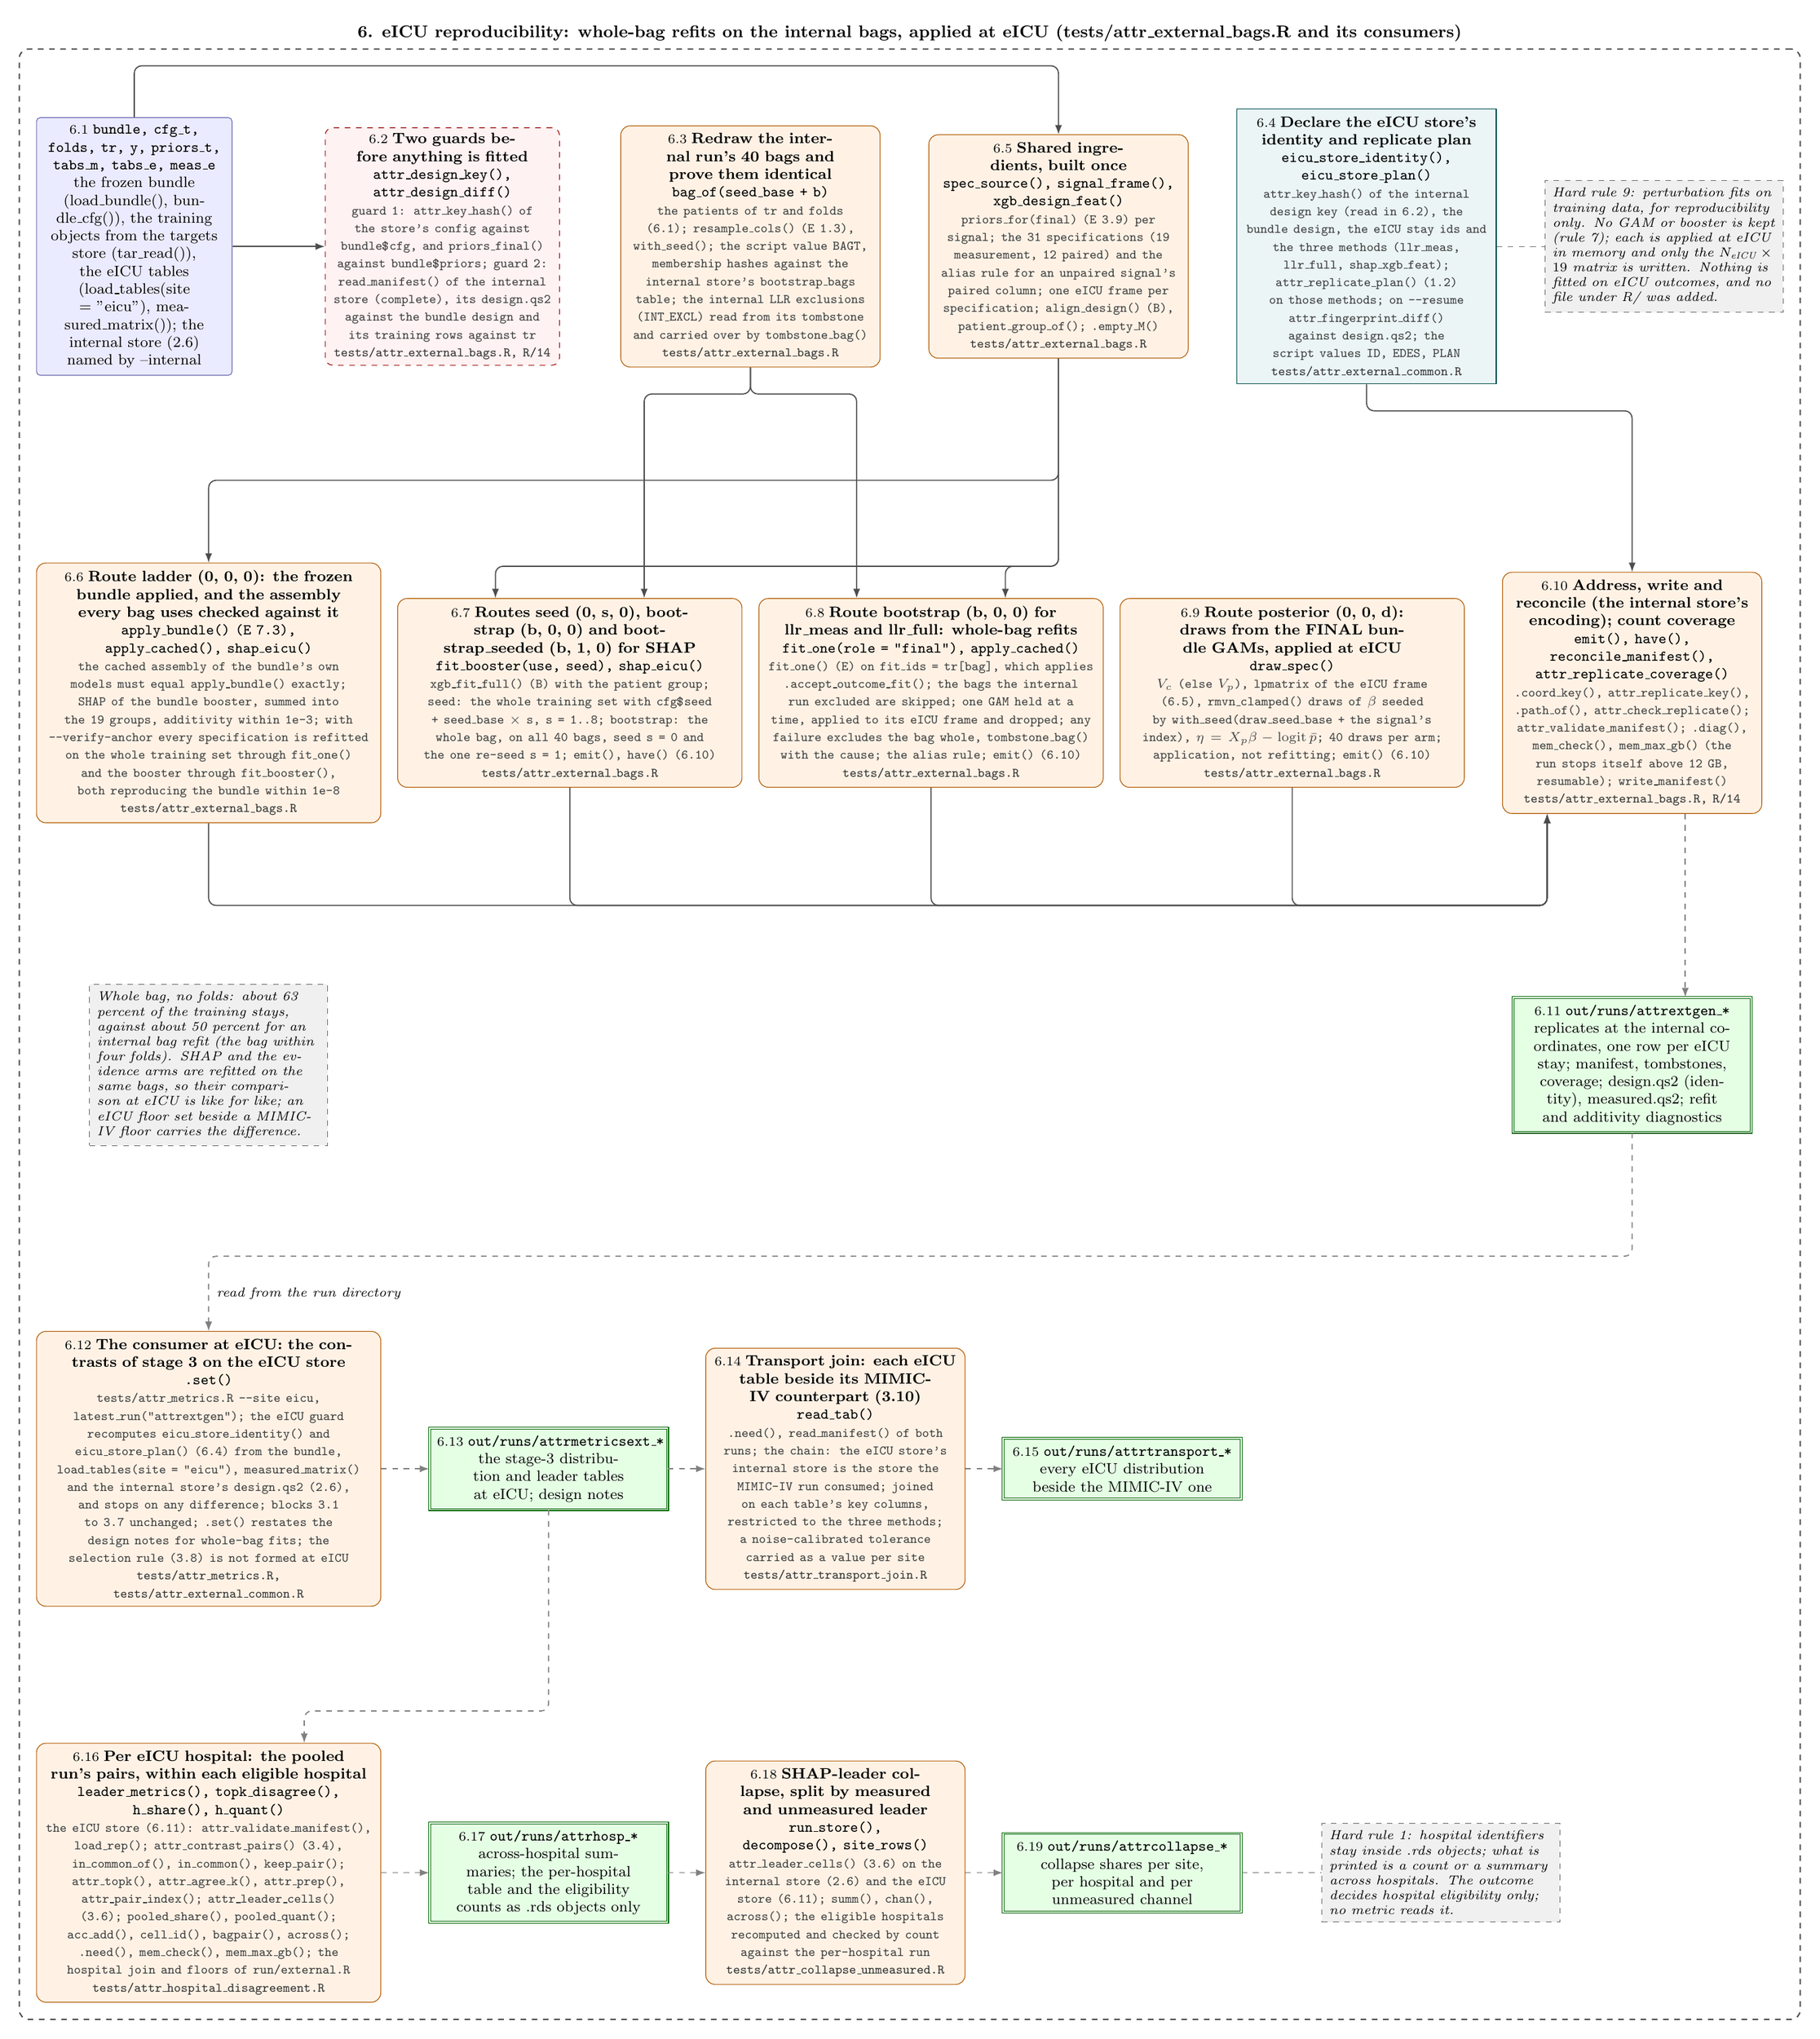
\begin{tikzpicture}[
  font=\footnotesize, x=1cm, y=1cm,
  fn/.style={draw=orange!70!black, fill=orange!10, rounded corners=5pt, align=center, inner sep=4pt, text width=4.6cm},
  fnw/.style={fn, text width=6.2cm},
  obj/.style={draw=blue!50!black!60, fill=blue!8, rounded corners=2pt, align=center, inner sep=4pt, text width=3.4cm},
  chk/.style={draw=red!60!black, fill=red!5, dashed, rounded corners=4pt, align=center, inner sep=3pt, text width=4.2cm},
  dcl/.style={draw=teal!60!black, fill=teal!8, align=center, inner sep=4pt, text width=4.6cm},
  outp/.style={draw=green!40!black, fill=green!10, double, align=center, inner sep=4pt, text width=3.6cm},
  note/.style={draw=black!60, dashed, fill=black!6, align=left, inner sep=4pt, text width=4.2cm, font=\scriptsize\itshape},
  e/.style={-{Latex[length=5pt]}, line width=0.6pt, draw=black!70, rounded corners=4pt},
  ex/.style={e, dashed, draw=black!50},
  en/.style={draw=black!55, dashed, line width=0.4pt},
  grp/.style={draw=black!70, dashed, line width=0.7pt, inner sep=9pt, rounded corners=5pt},
  lab/.style={font=\small\bfseries, anchor=south},
  al/.style={font=\scriptsize\itshape, fill=white, inner sep=1pt}]

\newcommand{\B}[5]{{\scriptsize #1}\;\textbf{#2}\\\texttt{\textbf{#3}}\\{\scriptsize\ttfamily\color{black!75}#4}\\{\scriptsize\ttfamily\color{black!80}#5}}
\newcommand{\Bs}[4]{{\scriptsize #1}\;\textbf{#2}\\\texttt{\textbf{#3}}\\{\scriptsize\ttfamily\color{black!80}#4}}
\newcommand{\Obj}[3]{{\scriptsize #1}\;\texttt{\textbf{#2}}\\#3}

% =====================================================================
% STAGE 6: the eICU reproducibility arm (attribution plan Part Seven):
% whole-bag refits on the internal bags, applied at eICU
% =====================================================================
\node[obj] (xin) at (2.8,-2.0) {\Obj{6.1}{bundle, cfg\_t, folds, tr, y, priors\_t, tabs\_m, tabs\_e, meas\_e}{the frozen bundle (load\_bundle(), bundle\_cfg()), the training objects from the targets store (tar\_read()), the eICU tables (load\_tables(site = "eicu"), measured\_matrix()); the internal store (2.6) named by --internal}};
\node[chk] (xguard) at (8.6,-2.0) {\B{6.2}{Two guards before anything is fitted}{attr\_design\_key(), attr\_design\_diff()}{guard 1: attr\_key\_hash() of the store's config against bundle\$cfg, and priors\_final() against bundle\$priors; guard 2: read\_manifest() of the internal store (complete), its design.qs2 against the bundle design and its training rows against tr}{tests/attr\_external\_bags.R, R/14}};
\node[fn]  (xbags) at (14.4,-2.0) {\B{6.3}{Redraw the internal run's 40 bags and prove them identical}{bag\_of(seed\_base + b)}{the patients of tr and folds (6.1); resample\_cols() (E 1.3), with\_seed(); the script value BAGT, membership hashes against the internal store's bootstrap\_bags table; the internal LLR exclusions (INT\_EXCL) read from its tombstone and carried over by tombstone\_bag()}{tests/attr\_external\_bags.R}};
\node[fn]  (xprep) at (20.2,-2.0) {\B{6.5}{Shared ingredients, built once}{spec\_source(), signal\_frame(), xgb\_design\_feat()}{priors\_for(final) (E 3.9) per signal; the 31 specifications (19 measurement, 12 paired) and the alias rule for an unpaired signal's paired column; one eICU frame per specification; align\_design() (B), patient\_group\_of(); .empty\_M()}{tests/attr\_external\_bags.R}};
\node[dcl] (xid) at (26.0,-2.0) {\B{6.4}{Declare the eICU store's identity and replicate plan}{eicu\_store\_identity(), eicu\_store\_plan()}{attr\_key\_hash() of the internal design key (read in 6.2), the bundle design, the eICU stay ids and the three methods (llr\_meas, llr\_full, shap\_xgb\_feat); attr\_replicate\_plan() (1.2) on those methods; on --resume attr\_fingerprint\_diff() against design.qs2; the script values ID, EDES, PLAN}{tests/attr\_external\_common.R}};
\node[note] (n10) at (31.6,-2.0) {Hard rule 9: perturbation fits on training data, for reproducibility only. No GAM or booster is kept (rule 7); each is applied at eICU in memory and only the $N_{\text{eICU}} \times 19$ matrix is written. Nothing is fitted on eICU outcomes, and no file under R/ was added.};

\node[fnw] (xanc) at (4.2,-10.4) {\B{6.6}{Route ladder (0, 0, 0): the frozen bundle applied, and the assembly every bag uses checked against it}{apply\_bundle() (E 7.3), apply\_cached(), shap\_eicu()}{the cached assembly of the bundle's own models must equal apply\_bundle() exactly; SHAP of the bundle booster, summed into the 19 groups, additivity within 1e-3; with --verify-anchor every specification is refitted on the whole training set through fit\_one() and the booster through fit\_booster(), both reproducing the bundle within 1e-8}{tests/attr\_external\_bags.R}};
\node[fnw] (xshap) at (11.0,-10.4) {\B{6.7}{Routes seed (0, s, 0), bootstrap (b, 0, 0) and bootstrap\_seeded (b, 1, 0) for SHAP}{fit\_booster(use, seed), shap\_eicu()}{xgb\_fit\_full() (B) with the patient group; seed: the whole training set with cfg\$seed + seed\_base $\times$ s, s = 1..8; bootstrap: the whole bag, on all 40 bags, seed s = 0 and the one re-seed s = 1; emit(), have() (6.10)}{tests/attr\_external\_bags.R}};
\node[fnw] (xllr) at (17.8,-10.4) {\B{6.8}{Route bootstrap (b, 0, 0) for llr\_meas and llr\_full: whole-bag refits}{fit\_one(role = "final"), apply\_cached()}{fit\_one() (E) on fit\_ids = tr[bag], which applies .accept\_outcome\_fit(); the bags the internal run excluded are skipped; one GAM held at a time, applied to its eICU frame and dropped; any failure excludes the bag whole, tombstone\_bag() with the cause; the alias rule; emit() (6.10)}{tests/attr\_external\_bags.R}};
\node[fnw] (xpost) at (24.6,-10.4) {\B{6.9}{Route posterior (0, 0, d): draws from the FINAL bundle GAMs, applied at eICU}{draw\_spec()}{$V_c$ (else $V_p$), lpmatrix of the eICU frame (6.5), rmvn\_clamped() draws of $\beta$ seeded by with\_seed(draw\_seed\_base + the signal's index), $\eta = X_p\beta - \operatorname{logit}\bar p$; 40 draws per arm; application, not refitting; emit() (6.10)}{tests/attr\_external\_bags.R}};
\node[fn]  (xstore) at (31.0,-10.4) {\B{6.10}{Address, write and reconcile (the internal store's encoding); count coverage}{emit(), have(), reconcile\_manifest(), attr\_replicate\_coverage()}{.coord\_key(), attr\_replicate\_key(), .path\_of(), attr\_check\_replicate(); attr\_validate\_manifest(); .diag(), mem\_check(), mem\_max\_gb() (the run stops itself above 12 GB, resumable); write\_manifest()}{tests/attr\_external\_bags.R, R/14}};

\node[note] (n11) at (4.2,-17.4) {Whole bag, no folds: about 63 percent of the training stays, against about 50 percent for an internal bag refit (the bag within four folds). SHAP and the evidence arms are refitted on the same bags, so their comparison at eICU is like for like; an eICU floor set beside a MIMIC-IV floor carries the difference.};
\node[outp, text width=4.2cm] (xgen) at (31.0,-17.4) {\Obj{6.11}{out/runs/attrextgen\_*}{replicates at the internal coordinates, one row per eICU stay; manifest, tombstones, coverage; design.qs2 (identity), measured.qs2; refit and additivity diagnostics}};

\node[fnw] (xmet) at (4.2,-25.0) {\B{6.12}{The consumer at eICU: the contrasts of stage 3 on the eICU store}{.set()}{tests/attr\_metrics.R --site eicu, latest\_run("attrextgen"); the eICU guard recomputes eicu\_store\_identity() and eicu\_store\_plan() (6.4) from the bundle, load\_tables(site = "eicu"), measured\_matrix() and the internal store's design.qs2 (2.6), and stops on any difference; blocks 3.1 to 3.7 unchanged; .set() restates the design notes for whole-bag fits; the selection rule (3.8) is not formed at eICU}{tests/attr\_metrics.R, tests/attr\_external\_common.R}};
\node[outp, text width=4.2cm] (xmetout) at (10.6,-25.0) {\Obj{6.13}{out/runs/attrmetricsext\_*}{the stage-3 distribution and leader tables at eICU; design notes}};
\node[fn]  (xjoin) at (16.0,-25.0) {\B{6.14}{Transport join: each eICU table beside its MIMIC-IV counterpart (3.10)}{read\_tab()}{.need(), read\_manifest() of both runs; the chain: the eICU store's internal store is the store the MIMIC-IV run consumed; joined on each table's key columns, restricted to the three methods; a noise-calibrated tolerance carried as a value per site}{tests/attr\_transport\_join.R}};
\node[outp, text width=4.2cm] (xjoinout) at (21.4,-25.0) {\Obj{6.15}{out/runs/attrtransport\_*}{every eICU distribution beside the MIMIC-IV one}};

\node[fnw] (xhosp) at (4.2,-32.6) {\B{6.16}{Per eICU hospital: the pooled run's pairs, within each eligible hospital}{leader\_metrics(), topk\_disagree(), h\_share(), h\_quant()}{the eICU store (6.11): attr\_validate\_manifest(), load\_rep(); attr\_contrast\_pairs() (3.4), in\_common\_of(), in\_common(), keep\_pair(); attr\_topk(), attr\_agree\_k(), attr\_prep(), attr\_pair\_index(); attr\_leader\_cells() (3.6); pooled\_share(), pooled\_quant(); acc\_add(), cell\_id(), bagpair(), across(); .need(), mem\_check(), mem\_max\_gb(); the hospital join and floors of run/external.R}{tests/attr\_hospital\_disagreement.R}};
\node[outp, text width=4.2cm] (xhospout) at (10.6,-32.6) {\Obj{6.17}{out/runs/attrhosp\_*}{across-hospital summaries; the per-hospital table and the eligibility counts as .rds objects only}};
\node[fn]  (xcol) at (16.0,-32.6) {\B{6.18}{SHAP-leader collapse, split by measured and unmeasured leader}{run\_store(), decompose(), site\_rows()}{attr\_leader\_cells() (3.6) on the internal store (2.6) and the eICU store (6.11); summ(), chan(), across(); the eligible hospitals recomputed and checked by count against the per-hospital run}{tests/attr\_collapse\_unmeasured.R}};
\node[outp, text width=4.2cm] (xcolout) at (21.4,-32.6) {\Obj{6.19}{out/runs/attrcollapse\_*}{collapse shares per site, per hospital and per unmeasured channel}};
\node[note] (n12) at (27.4,-32.6) {Hard rule 1: hospital identifiers stay inside .rds objects; what is printed is a count or a summary across hospitals. The outcome decides hospital eligibility only; no metric reads it.};

% generator: inputs, guards, ingredients, identity
\draw[e] (xin) -- (xguard);
\draw[e] (xin.north) |- (20.2,1.4) -- (xprep.north);
\draw[en] (xid.east) -- (n10.west);
% the bags reach the bootstrap routes; the ingredients reach the routes that refit or assemble
\draw[e] (xbags.south) -- ++(0,-0.5) -| ($(xshap.north)+(1.4,0)$);
\draw[e] (xbags.south) -- ++(0,-0.5) -| ($(xllr.north)+(-1.4,0)$);
\draw[e] (xprep.south) |- (4.2,-6.4) -- (xanc.north);
\draw[e] (xprep.south) |- ($(xshap.north)+(-1.4,0.6)$) -- ($(xshap.north)+(-1.4,0)$);
\draw[e] (xprep.south) |- ($(xllr.north)+(1.4,0.6)$) -- ($(xllr.north)+(1.4,0)$);
\draw[e] (xid.south) -- ++(0,-0.5) -| (xstore.north);
% every route writes through 6.10
\draw[e] (xanc.south) |- (29.4,-14.4) -- ($(xstore.south)+(-1.6,0)$);
\draw[e] (xshap.south) |- (29.4,-14.4) -- ($(xstore.south)+(-1.6,0)$);
\draw[e] (xllr.south) |- (29.4,-14.4) -- ($(xstore.south)+(-1.6,0)$);
\draw[e] (xpost.south) |- (29.4,-14.4) -- ($(xstore.south)+(-1.6,0)$);
\draw[ex] ($(xstore.south)+(1.0,0)$) -- ($(xgen.north)+(1.0,0)$);
% the consumers, each reading the run directories before it
\draw[ex] (xgen.south) |- (4.2,-21.0) -- (xmet.north) node[al, pos=0.5, anchor=west] {~read from the run directory};
\draw[ex] (xmet) -- (xmetout); \draw[ex] (xmetout) -- (xjoin); \draw[ex] (xjoin) -- (xjoinout);
\draw[ex] (xmetout.south) |- ($(xhosp.north)+(1.8,0.6)$) -- ($(xhosp.north)+(1.8,0)$);
\draw[ex] (xhosp) -- (xhospout); \draw[ex] (xhospout) -- (xcol); \draw[ex] (xcol) -- (xcolout);
\draw[en] (xcolout.east) -- (n12.west);

\begin{scope}[on background layer]
\node[grp, fit={(xin)(xguard)(xbags)(xid)(n10)(xprep)(xanc)(xshap)(xllr)(xpost)(xstore)(xgen)(n11)(xmet)(xmetout)(xjoin)(xjoinout)(xhosp)(xhospout)(xcol)(xcolout)(n12)(20.2,1.4)}, label={[lab]north:{6. eICU reproducibility: whole-bag refits on the internal bags, applied at eICU (tests/attr\_external\_bags.R and its consumers)}}] (b6) {};
\end{scope}
\end{tikzpicture}
\end{document}
